\section{Experiments}\label{sec:experiments}

We report an executable artefact, a deterministic zero-model ablation with
pre-registered hypotheses, and an illustrative real-host pilot.

\subsection{Artifact and reproducibility}\label{sec:exp:artifact}

The engine is zero-dependency Python with no model calls; the plugin is a
JavaScript re-implementation. Feasibility is asserted: 892 Python assertions over
14 test files and 396 plugin assertions (188/148/45/15), the latter count taken
at the 2026-10-27 audit snapshot and not re-executed for this paper. Re-executed
here for
Section~\ref{sec:method}: 161, 65 and 26 assertions, all pass. Three drift
checks were green at submission: a 66-key rule/engine/plugin comparison, a
contract digest, and an implementation-status matrix check. Determinism is
enforced: fixed clock (60\,s per turn), no wall clock, no randomness, no
network. Same configuration, store and script give byte-identical runs; this run
reports \texttt{model\_calls=0}, \texttt{network\_calls=0}, two written files and
51/51 verifier checks.

\subsection{Deterministic three-arm ablation}\label{sec:exp:ablation}

\paragraph{Protocol.} A 100-turn script is generated deterministically from the
chaos and replay corpora (SHA-256 \texttt{701ff06a0b37\ldots}): 21,610 characters
against a 24,000-character window, maximum usage ratio $0.9004$, with the
phase-shift monitor firing on turns 73--100 (28 turns). Twelve probes cover
long-range settings (A), superseded values (B), distractor-overloaded settings
(C), and a constructed high-frequency-old preference (D, 30 accesses ending 100
days ago); two no-hit probes sit at turns 86--87. Hits are decided by entry
sensitivity. \textsc{Baseline} injects the last three raw turns with no memory or
control layer; \textsc{Basic} uses budgeted query-conditioned recall with the
ACT-R channel off (\texttt{actrWeight=0}), static weights and no control layer;
\textsc{Full} uses defaults, i.e.\ both potency channels, dynamic weights and all
four control subsystems. Harness and pipeline agree on 100/100 turns for the
wire-compatible core; label-on divergences are recorded in the result file.
Table~\ref{tab:ablation} and Figure~\ref{fig:retention} report the outcomes.

\begin{table*}[t]
\centering\footnotesize
\caption{Three-arm ablation. SFR: setting-forgetting rate per class and overall;
NHD: no-hit discipline (literal variant in parentheses); IIR: adversarial
interference ratio; telemetry: phase/anchor turns, fallback marks (actual drops),
UCA-08 records. Source:
\texttt{results/abl-20261027-003626-engine.json}, fields
\texttt{conditions.<arm>.metrics.*} and \texttt{conditions.<arm>.telemetry.*};
verifier 51/51.}
\label{tab:ablation}
\begin{tabular}{@{}l cccc c c c c c ccc c@{}}
\toprule
 & \multicolumn{4}{c}{SFR by probe class} & & & & & & \multicolumn{3}{c}{Jailbreak (\%)} & \multicolumn{1}{c}{Telemetry}\\
\cmidrule(lr){2-5}\cmidrule(lr){11-13}\cmidrule(lr){14-14}
Arm & A & B & C & D & SFR$_{\text{text}}$ [95\% CI] & SFR$_{\text{id}}$ & IIR & NHD & UCE & in & fp & script & ph/anc/fb/08 \\
\midrule
Baseline & 1.00 & 1.00 & 1.00 & 1.00 & 1.00$^{\ddagger}$ & $\varnothing$ & $\varnothing$ & $\varnothing$ & $0^{\dagger}$ & $\varnothing$ & $\varnothing$ & $\varnothing$ & 0/0/0/0 \\
Basic & 0.00 & 0.00 & 0.00 & 1.00 & 0.25 [0.05, 0.57] & 0.25 & 0.56 & 1.00 (0.00) & $0^{\dagger}$ & $\varnothing$ & $\varnothing$ & $\varnothing$ & 0/0/0/0 \\
Full & 0.00 & 0.00 & 0.00 & 0.00 & 0.00 [0.00, 0.26] & 0.00 & 0.47 & 1.00 (0.00) & $0^{\dagger}$ & 1.00 (25) & 0.00 (294) & 0.00 (6) & 28/28/4(0)/62 \\
\bottomrule
\end{tabular}

\vspace{2pt}
\raggedright\scriptsize
$\varnothing$: not applicable; the cell is \texttt{null} with a reason, never
zero. $^{\ddagger}$: by construction---a three-turn window cannot contain a
setting planted 85 turns earlier. $^{\dagger}$:
structurally zero, since all injected items are active and user-explicit.
\end{table*}

\paragraph{Results.} Both LINGSHU arms retrieve the nine A/B/C probes perfectly,
and the baseline's $1.00$ is window arithmetic---definitional by construction---so
we do not treat the baseline--system difference as an effect size. The arms separate only on class D:
\textsc{Basic} misses all three, \textsc{Full} retrieves all three, giving $0.25$
versus $0.00$ ($p=0.125$, three discordant pairs, not significant). With twelve
paired probes the exact sign test detects only a $5/12\approx0.42$ difference at
$\alpha=0.05$ ($6/12=0.50$ after Bonferroni correction), and a three-item class
cannot reach significance at all; we therefore report direction and per-probe
detail only. Order permutations leave SFR unchanged but move anchor counts
(28/62/21): retention is order-robust, phase timing is not.

Pre-registered outcomes are reported with failures. P1b passes on its point
estimate but fails its confidence criterion (Basic's Clopper--Pearson upper bound
is $0.572$ against a required $0.45$). P2 passes under the code-faithful
predicate, while the literal substring predicate returns $0.00$ because the
engine's wording differs; both numbers stand. P3 is not evaluable, as both arms
are structurally zero. P5 is undecidable:
in-distribution jailbreaks are blocked 25/25, false positives are 0/294 and
scripted user-turn jailbreaks 0/6, but the held-out set was never
authored, so that cell is \texttt{null}. P6 passes (28 phase turns, 28
anchors, 4 fallback marks, 62 UCA-08 records for \textsc{Full}; all zero for
\textsc{Basic}). P7 passes for single-anchor overhead ($+100$ to $+124$
characters) but fails its literal two-times threshold.

\paragraph{Reading the phase window.} Both thresholds fall inside the run: the
ratio crosses $0.70$ at turn 73 (phase \emph{shift}) and $0.85$ at turn 85 (phase
\emph{critical}), so the shift window is turns 73--100 and the critical window
turns 85--100 (Section~\ref{sec:method:phase}). The telemetry shows what the
thresholds change in practice, not only in the formula: \textsc{Full} records 28
phase turns and 28 anchors with 4 fallback marks and 62 UCA-08 records, while
\textsc{Basic} records 0/0/0/0, and the anchor strip under Figure~\ref{fig:retention}
begins at turn 73 and continues through the critical window. The figure also shows
why the phase monitor cannot improve retention by itself: \textsc{Basic} and
\textsc{Full} have identical injected sets, so the shaded bands mark when the
control plane starts paying a prompt-budget cost, not when memory improves. We
therefore read the 70\%/85\% thresholds as escalation points for anchoring and
audit, not as learning or retrieval gains.

\subsection{Real-host pilot}\label{sec:exp:host}

Ten cells ran on one host and one model route, one run each. The details are in
Appendix~\ref{app:hostpilotdata}; the methodological finding is that compressing
a 100-turn dialogue into one 78\,KB request dilutes the query until
query-conditioned retrieval stops hitting (\textsc{Full} reports \texttt{matched=0}),
and the control layer never fired in any cell (the gate returned \texttt{allow}
with an empty UCA list throughout). This is a mechanism demonstration at $n=1$,
not a hallucination rate.

\begin{figure*}[t]
\centering
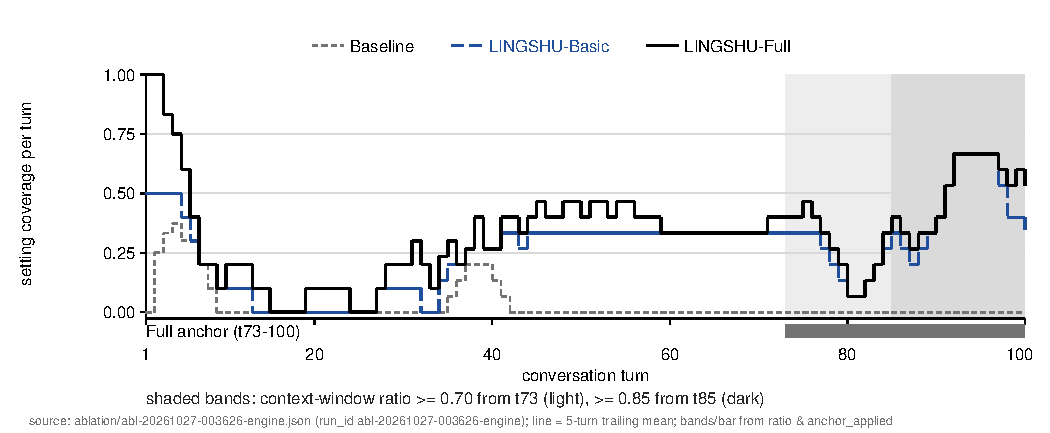
\includegraphics[width=\textwidth]{figures/fig2-retention.pdf}
\caption{Setting coverage per turn over the 100-turn script:
$y_t = |\mathcal{S}^{\mathrm{inj}}_t \cap \mathcal{S}^{\mathrm{act}}_t| /
|\mathcal{S}^{\mathrm{act}}_t|$, the fraction of currently active planted
settings that appear in the injected context (plotted as a 5-turn trailing mean;
the raw turn means are 0.025, 0.260 and 0.327 for
Baseline, Basic and Full). Basic and Full overlap by design: the control plane
does not change retrieval membership. Shaded bands mark the phase-shift window
($r \ge 0.70$ from turn 73, $r \ge 0.85$ from turn 85); the strip below the axis
marks turns on which Full injects head/tail persona anchors. Source:
\texttt{conditions.<arm>.turns[].\{setting\_ids\_injected, active\_setting\_ids,
ratio, anchor\_applied\}} in \texttt{abl-20261027-003626-engine.json}.}
\label{fig:retention}
\end{figure*}

\subsection{Robustness under Chaos Injection}\label{sec:exp:chaos}

\paragraph{Protocol.} Three faults are injected from \emph{outside} the system;
\texttt{plugin/}, \texttt{engine/} and \texttt{rules/} are hashed before and
after the campaign and are unchanged. Each case runs in its own \texttt{DSH\_HOME}
whose profile copy links (via a directory junction) to the repository plugin, so
the measured code is the current reference implementation and the injection is
confined to the host layer and to on-disk memory state. All runs are headless CLI
invocations with a fixed short prompt; transcripts, plugin state, audit logs and
final prompts are written to disk and analysed offline. One injected point is run
once ($n=1$); no red-team mutation is performed in this section.

\emph{A, transport faults.} The host's model endpoint is redirected through the
documented \texttt{DEEPSEEK\_BASE\_URL} environment variable to a local mock that
returns HTTP 500, a valid but empty 200 response, a valid 200 response carrying a
fabricated answer, or accepts the connection and never answers.

\emph{B, memory faults.} The memory store is corrupted at the file level, without
touching \texttt{memorywriter.js}: (B1) \texttt{memory.jsonl} is replaced by a
directory, so reads fail with \texttt{EISDIR} and are swallowed while writes throw;
(B2) a readable but dirty store is seeded with a torn JSON line, a duplicate id
whose later row is a supersession tombstone, and two active rows that share
$(\textsc{subject},\textsc{relation})$ but disagree on \textsc{object}. A warm-state
template is pre-seeded so that the cold-start gate does not mask the effect; this
setup is synthetic and disclosed as such.

\emph{C, context flood.} A deterministic 150{,}000-character garbage stream
($\approx 50$k tokens at the plugin's 3-chars/token estimator) is passed as the
user message while \texttt{LINGSHU\_CONTEXT\_WINDOW} fixes the plugin's perceived
window at four values; a mock endpoint records the assembled request body, so the
run costs no model tokens.

\begin{table*}[t]
\centering\footnotesize
\caption{Fault-injection matrix. Every cell is an observed value from one run;
$\varnothing$ marks a quantity the injected fault makes inapplicable, never zero.
A: five transport modes on one fixed prompt. B: three headless runs on a synthetic
warm state. C: four window values on the same 150k-character input plus exact
boundary brackets. Source: \texttt{experiments/chaos-injection/out/}.}
\label{tab:chaos}
\begin{tabular}{@{}l l l l@{}}
\toprule
Fault & Injected mode & Control-plane observation & Key numbers \\
\midrule
A transport & HTTP 500 & error surfaced by host; injection still ran once & 7 tries, 17.99 s, exit 1 \\
            & empty 200 & empty final message passed through, exit 0 & final length 0 \\
            & fabricated 200 & fabricated text reached stdout, exit 0 & final length 23 \\
            & never answers & no client-side timeout inside 150 s window & $\ge$150.03 s \\
            & all modes & \texttt{blocked=false}; constitution in prompt & 5/5 \\
B memory    & store as directory (B1) & \texttt{hook\_error}=1 (\texttt{EISDIR}); writes 0; reply returned & 9.851 s, exit 0 \\
            & dirty store (B2) & \texttt{fallback=true}, \texttt{drop style}; superseded not recalled & 21.046 s, exit 0 \\
            & clean control (B0) & style and organization injected; no fallback & 45.654 s, exit 0 \\
C context   & 4 windows, 150k chars & \texttt{normal/shift/shift/critical}; constitution 4/4 & ratios 0.681/0.701/0.721/0.851 \\
            & boundary brackets & \texttt{0.7000}$\to$normal, \texttt{0.7006}$\to$shift; \texttt{0.8500}$\to$shift, \texttt{0.8507}$\to$critical & 8 headless calls, 0 model calls \\
\bottomrule
\end{tabular}
\end{table*}

\paragraph{Transport faults (A).} A plain 200 response completes in 2.84\,s. An
HTTP 500 is retried by the host seven times with exponential backoff
(0.55, 0.96, 1.92, 4.25, 7.51\,s between attempts) and surfaces one error line
(\texttt{dsh: SERVER: mock upstream 500}) after 17.99\,s, exiting non-zero with
\emph{no} fabricated text. An endpoint that never answers produces no response
within a 150\,s observation window and is terminated by the harness, not by a
client timeout. In all five modes the plugin performed exactly one pre-step
injection, the constitution section remained in the final prompt,
\texttt{state.control.blocked} stayed false and no hook error was recorded. An
empty 200 response was passed through as an empty final message (exit 0), and a
fabricated 200 response reached stdout verbatim (23 characters). The control plane
therefore never converts a transport failure into fabricated content, but it adds
neither a transport timeout nor an output validator: those remain host-layer
responsibilities.

\paragraph{Memory faults (B).} With a clean store (B0) the injected prompt carries
constitution, metacognition, organization and style sections and no fallback mark.
Replacing the store by a directory (B1) raises one \texttt{hook\_error}
(\texttt{Error: EISDIR ... write}) and leaves \texttt{stateWrites} at its
pre-run value, yet the turn still exits 0 and returns a 364-character answer with
the constitution and style sections intact---feature fail-open, memory isolated.
Two caveats are reported rather than smoothed over: the reply asserts that the
fact was recorded although the write demonstrably failed, and the model's
own status narration quotes the synthetic warm-template counter, so only on-disk
evidence is used for judgement. With the dirty store (B2) recall returns
\texttt{mem\_002} and \texttt{mem\_003} while the superseded tombstone
\texttt{mem\_001} is absent; the conflict on the
$(\textsc{subject},\textsc{relation})$ pair is classified
unresolved, the variety guard sets \texttt{fallback=true} with
\texttt{dropDomains=["style"]}, the final prompt loses its style section but keeps
the conflict-to-clarify marker and the constitution block, \texttt{verdict} remains
\texttt{allow} and \texttt{blocked} false, and the model asks the user to
disambiguate instead of choosing a value. The dirty store also exposes a
rule-stub artefact: the \emph{question} ``what is my project codename?'' is
extracted as a fact whose object is the interrogative ``what'', and in B2 its
write supersedes both conflicting rows
(\texttt{supersedeEvents}=2). That artefact must not be read as a benefit: it
means the next turn's conflict can be erased by the query itself.
\footnote{The byte-exact CJK prompt markers and conflict keys are recorded
verbatim in \texttt{experiments/chaos-injection/out/}; this paper renders them in
ASCII so that the source compiles with the standard T1 fonts.}

\paragraph{Context flood (C).} Measured usage ratios (four decimals) are 0.6806,
0.7006, 0.7206 and 0.8507 for the four windows; the phase is
\texttt{normal}, \texttt{shift}, \texttt{shift}, \texttt{critical} respectively.
Two exact boundary brackets pin the thresholds: under $\ge$ semantics the largest
shifting window is 71{,}490 ($r=0.700000$), and 71{,}491 is \texttt{normal};
the largest critical window is 58{,}874 ($r=0.8500017$) and 58{,}875 is
\texttt{shift}. Four-decimal display is a trap: window 71{,}493 prints
\texttt{0.7000} yet stays \texttt{normal}, and 58{,}876 prints \texttt{0.8500}
yet stays \texttt{shift}; only the unrounded ratio is decisive. The plugin's
estimate is 50{,}043 tokens for a nominal 50{,}000: its input is the 150{,}127-character
JSON message envelope (127 characters of \texttt{role}/\texttt{content} wrapping),
so all measured ratios sit $\approx 0.0006$ above their nominal values. The host
then renders 151{,}936 JSON characters (50{,}646 tokens), appending a
1{,}809-character instruction block to the user message; the plugin therefore
under-estimates model-visible input by about $1.2\%$. Physical occupancy is
$\approx 5.2\%$ of the model's 1M-token window: the window here is a laboratory
override, and the ratio is a relative control signal rather than a saturation
measurement.

No truncation occurs: in 4/4 runs the full input appears in the mock request body
(\texttt{prompt\_full\_in\_body}), the truncation rate is 0.0, and the constitution
section is present in 4/4 requests. Anchor delivery, however, exposes a genuine
one-assembly lag. The plugin's own prompt preview carries a head anchor whenever
\texttt{prefeed} is set and both head and tail anchors once \texttt{critical};
the \emph{request} reaching the model carries the anchor set of the \emph{previous}
turn in 8/8 observed requests. The clearest case is the first \texttt{critical}
turn: its preview has head and tail, its request has only the head, and only the
next request carries both. The mechanism is host-side: the agent loop assembles the
system prompt before it emits \texttt{agent/pre-step}, where the plugin updates the
phase state (assembly precedes the hook by four source lines in
\texttt{dsh-agent-loop}); the plugin cannot rewrite the already-composed request.
Even when delivered, the tail anchor ends at system offset 229 of 2{,}906 characters,
i.e.\ at roughly $0.17\%$ of the model-visible text, so ``head and tail'' means
sections 90/140 of the plugin's seven-part prompt, not the absolute ends of the
request. A single-turn or single-shot deployment should therefore not expect
critical anchors to take effect on the turn that produces the critical ratio.

\begin{figure*}[t]
\centering
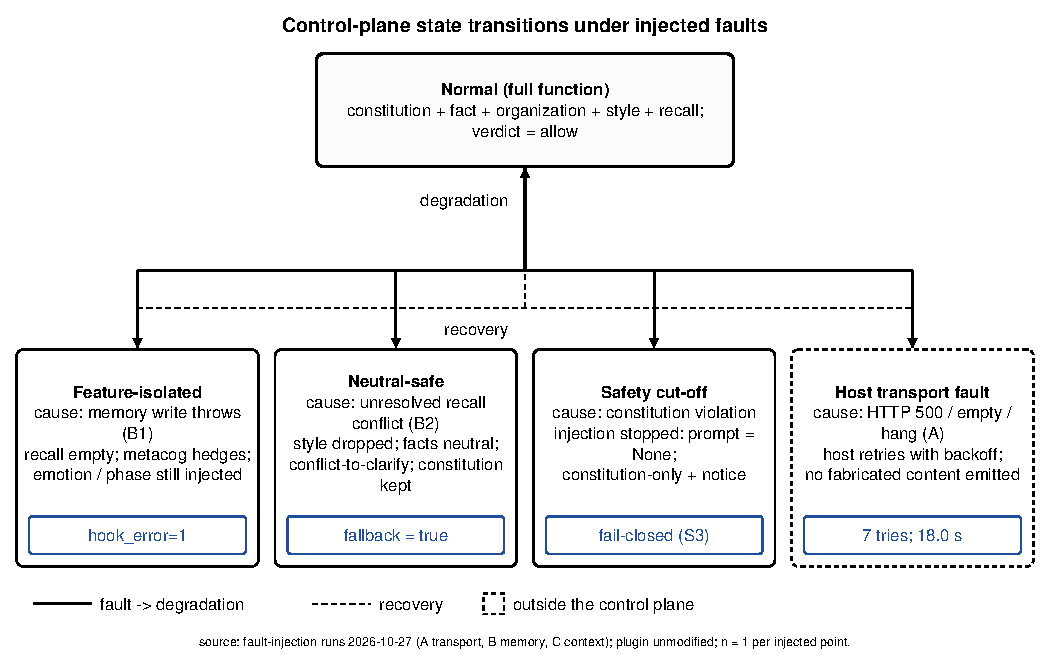
\includegraphics[width=0.98\textwidth]{figures/fig3-robustness.pdf}
\caption{Control-plane state transitions under injected faults. Normal operation
degrades along three distinct paths---feature isolation under a memory write
failure (B1), neutral-safe output under an unresolved recall conflict (B2), and
the security cut-off under a constitution violation (the existing STPA evidence
in \texttt{docs/22})---while transport faults remain outside the control plane
(A). Solid arcs are fault-to-degradation transitions, dashed arcs are recoveries.
Per-point evidence and the exact numbers are in
\texttt{experiments/chaos-injection/out/}; $n=1$ per injected point, plugin
unmodified.}
\label{fig:chaos}
\end{figure*}

\paragraph{What the asymmetry guarantees.} Across the three scenarios the control
plane behaves asymmetrically in exactly one direction: when a \emph{security}
predicate is at stake the gate is fail-closed and stops injection rather than
softening refusal, while when a \emph{feature} is at stake the failure is
fail-open---memory isolation and neutral-safe output keep the turn usable, the
constitution block is preserved and no fault is silently converted into
content---so \emph{LINGSHU's asymmetric degradation mechanism (fail-closed for
security, fail-open for features) ensures system availability under extreme
chaos}. The scope of that sentence is the control plane. Transport faults are
surfaced but neither timed out nor retried by the plugin, model output is not
validated by the plugin, and one B1 reply asserted a persistence that did not
happen; availability under transport faults therefore depends on the host, and
output truthfulness remains outside the mechanism's remit.

\subsection{Scope of the evidence}\label{sec:exp:notshow}

These experiments establish contract behaviour and mechanism reachability, not
model-level effect sizes: the engine is model-free, the host runs are one run per
cell on one model route, and the chaos faults are $n=1$ synthetic injections
rather than a sample of production failures. Two structural limits are worth
naming here because they shape the claims: the anchor set that reaches the model
lags the plugin's phase by one assembly, so the first critical request carries
only the head anchor; and host runs involve a real model and are therefore not
deterministic, which is why every claim above is tied to a field in the evidence
files rather than to a summary sentence. The full itemised list of parameter,
sample and environment limits is consolidated in Section~\ref{sec:limitations}.
